%%%%%%%%%%%%%%%%%%%%%%%%%%%%%%%%%%%%%%%%
%% MCM/ICM LaTeX Template %%
%% 2023 MCM/ICM           %%
%%%%%%%%%%%%%%%%%%%%%%%%%%%%%%%%%%%%%%%%
\documentclass[12pt]{article}
\usepackage{geometry}
\geometry{left=1in,right=0.75in,top=1in,bottom=1in}

%%%%%%%%%%%%%%%%%%%%%%%%%%%%%%%%%%%%%%%%
% Replace ABCDEF in the next line with your chosen problem
% and replace 1111111 with your Team Control Number
\newcommand{\Problem}{C}
\newcommand{\Team}{2322161}
\newcommand\keywords[1]{\textbf{Keywords}: #1}
 
%%%%%%%%%%%%%%%%%%%%%%%%%%%%%%%%%%%%%%%%

\usepackage{newtxtext}
\usepackage{amsmath,amssymb,amsthm}
\usepackage{newtxmath} % must come after amsXXX

\usepackage[pdftex]{graphicx}
\usepackage{xcolor}
\usepackage{fancyhdr}
\usepackage{tablefootnote}
\lhead{Team \Team}
\rhead{}
\cfoot{}

\newtheorem{theorem}{Theorem}
\newtheorem{corollary}[theorem]{Corollary}
\newtheorem{lemma}[theorem]{Lemma}
\newtheorem{definition}{Definition}

%%%%%%%%%%%%%%%%%%%%%%%%%%%%%%%%
\begin{document}
\graphicspath{{.}}  % Place your graphic files in the same directory as your main document
\DeclareGraphicsExtensions{.pdf, .jpg, .tif, .png}
\thispagestyle{empty}
\vspace*{-16ex}
\centerline{\begin{tabular}{*3{c}}
	\parbox[t]{0.3\linewidth}{\begin{center}\textbf{Problem Chosen}\\ \Large \textcolor{red}{\Problem}\end{center}}
	& \parbox[t]{0.3\linewidth}{\begin{center}\textbf{2023\\ MCM/ICM\\ Summary Sheet}\end{center}}
	& \parbox[t]{0.3\linewidth}{\begin{center}\textbf{Team Control Number}\\ \Large \textcolor{red}{\Team}\end{center}}	\\
	\hline
\end{tabular}}

%%%%%%%%%%%%%%%%%%%%%%%%%%%%%%%%%%%%%%%%

\newcommand{\subsubsubsection}[1]{\paragraph{#1}\mbox{}\\}
\setcounter{secnumdepth}{4} % how many sectioning levels to assign numbers to
\setcounter{tocdepth}{4} % how many sectioning levels to show in ToC

%%%%%%%%%%% Begin Summary %%%%%%%%%%%
\vspace{0.5cm}
{\Large
\centerline{\textbf{Predicting Wordle Results}}}

\vspace{0.3cm}
{\large
\centerline{\textbf{Summary}}}

\vspace{0.3cm}
\noindent
Wordle is a popular puzzle game on the Internet. It receives a lot of attention and raises a lot of discussions on Twitter. In this article, we analyze the daily report results from Twitter and predict future user volume and gaming results.

\vspace{0.3cm}
\noindent
In Model \uppercase\expandafter{\romannumeral1}, we establish a mathematical model describing the population growth of the game. We generate a Mathematical Time Series Wordle Prediction Model by combining the Logarithmic Normal and Logistic Growth Models. Using the model, we successfully predicted the number of reported results on March 1, 2023.

\vspace{0.3cm}
\noindent
We construct a Monte Carlo Simulation Model in Model \uppercase\expandafter{\romannumeral2} to simulate the Wordle process. This model contains three algorithms responsible for judgment, selection, and processing. Using this model, we obtain a prediction dataset for all the words that appear in the reported data. The prediction dataset shows homogeneity with the reported data. Then we use the model to predict the word "EERIE".

\vspace{0.3cm}
\noindent
In Model \uppercase\expandafter{\romannumeral3}, using the K-Means and Gaussian Mixture Model, we build a clustering model to determine the best number of clusters and classify the difficulty into three levels. By comparison, K-Means Model offers a better accuracy on the samples. We can predict the difficulty using our model and the generated prediction distribution from Model \uppercase\expandafter{\romannumeral2} of the word "EERIE".

\vspace{0.3cm}
\noindent
Finally, we conclude and write a letter to the Puzzle Editor to report our models and corresponding answers to the questions asked by the New York Times.

\vspace{0.3cm}
\noindent
\begin{keywords}
Logarithmic Normal Model; Logistic Growth Model; Monte Carlo Simulation Model; Random Forest Classification Model; K-Means Clustering Model; Gaussian Mixture Model;
\end{keywords}
%%%%%%%%%%% End Summary %%%%%%%%%%%

%%%%%%%%%%%%%%%%%%%%%%%%%%%%%%
\clearpage
\pagestyle{fancy}
% Uncomment the next line to generate a Table of Contents
%\tableofcontents 
\newpage
\setcounter{page}{1}
\rhead{Page \thepage\ }
%%%%%%%%%%%%%%%%%%%%%%%%%%%%%%

\tableofcontents
\vspace{0.3cm}
\noindent
\textbf{References\quad\quad\quad\quad\quad\quad\quad\quad\quad\quad\quad\quad\quad\quad\quad\quad\quad\quad\quad\quad\quad\quad\quad\quad\quad\quad\quad\quad\quad\quad\quad\quad\quad\quad\;\;\,\,\,21}
\newpage

\section{Introduction}
\subsection{Problem Background}
Wordle is an online puzzle provided by the New York Times. The popular game is updated daily and requires players to fill in a five-letter word puzzle with a maximum of six opportunities each day. Three colors denote denote the states of the game process. For instance, a green tile indicates the letter and word are in the correct position. A yellow tile shows that the letter belongs to the word but is in the wrong position. And a gray tile indicates that the letter isn't in the word. Figure\ref{wordle} shows the corresponding color tiles. Moreover, a "Hard Mode" increased the difficulty by forcing players to include their correct guesses (tiles in green or yellow) in the next tries.

\begin{figure}[h]
    \centering
    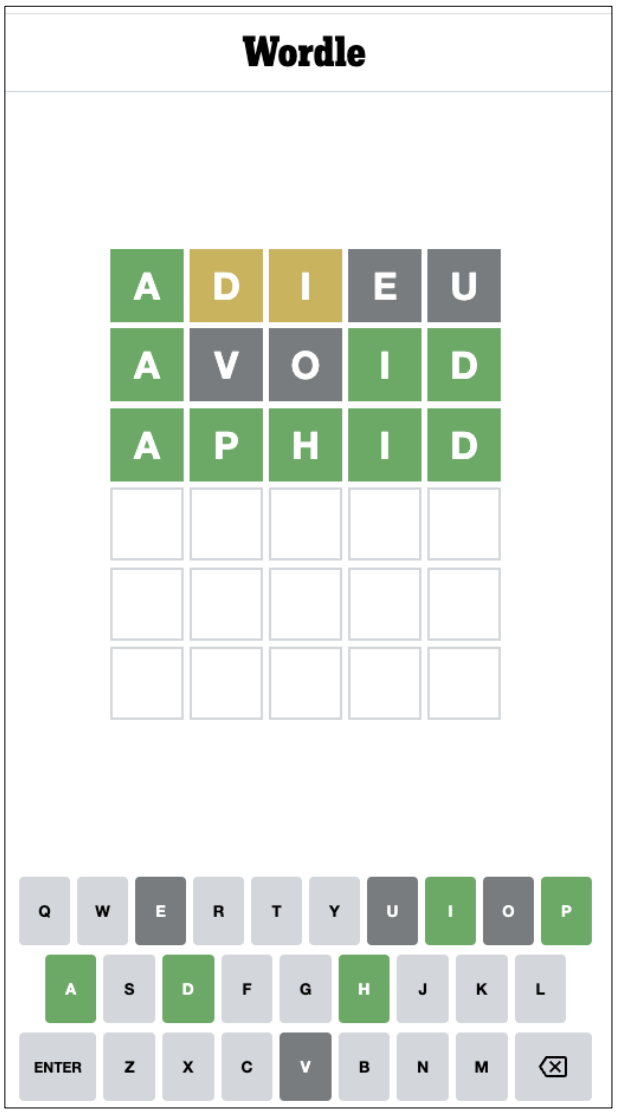
\includegraphics[width=7.5cm]{figures/wordle.png}
    \caption{Wordle Game Interface}
    \label{wordle}
\end{figure}

\vspace{0.3cm}
\noindent
Many users are sharing their scores on a social media named Twitter. Figure~\ref{twitter} is an example. Daily reports from January 7, 2022 to December 31, 2022 are given, which includes the date, contest number, word of the day, the number of people reporting scores that day, the number of players on hard mode, and the percentage that guessed the word from one to six tries, or could not solve the puzzle (denoted by X). 

\begin{figure}[h]
    \centering
    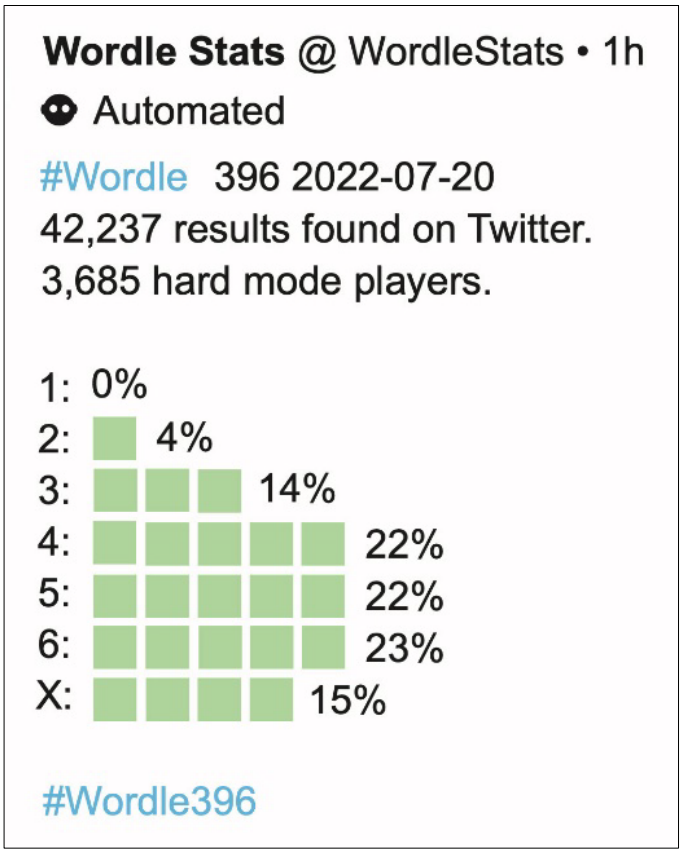
\includegraphics[width=7.5cm]{figures/twitter.png}
    \caption{Twitter Report Example}
    \label{twitter}
\end{figure}

\subsection{Restatement of the Problem}
According to the data provided by MCM and information identified in the problem statement, we need to establish several models and complete the following tasks with the models:

\begin{itemize}
  \item {Develop a model to explain the daily variation of the report results and create a prediction interval on March 1, 2023. Also, determine and explain whether the attributes of the word affect the percentage of scores reported that were played in Hard Mode.}
  \item {Predict the distribution of the report results based on a model and a given target word EERIE on March 1, 2023. The analysis gives the uncertainties and confidence of the model's prediction results.}
  \item {Summarize a model to make word classification based on their difficulty, using the attributes of a given word "EERIE" for classification. Meanwhile, discuss the accuracy of the classification.}
  \item {Display and explain some other interesting features of the report results dataset.}
  \item {Design a one- to two-page letter to the Puzzle Editor of the New York Times to summarize the results.}
\end{itemize}

\section{Assumptions and Justifications}

Assumptions are made as follows to simply the problem, each of which is appropriately justified.

\begin{itemize}
    \item {\textbf{Assumption 1:} Assuming the players are rational and devoted, they will try their best to solve the puzzle based on the condition.}
    
    \textbf{Justification:} Rational users tend to take a predictable  and feasible approach to solving the Wordle puzzle, which means their gaming pattern can be tracked and modeled. We need to add this restriction to better fit our model into the dataset to simplify the circumstance.
    \item {\textbf{Assumption 2:} Assuming the players are honest, the report results are highly credible.}
    
    \textbf{Justification:} Although fake information on social media exists in the real world, the problem requires us to generate a prediction model based solely on the information provided. With this assumption, we can analyze the results correctly.
    \item {\textbf{Assumption 3:} Assuming users' average level (e.g. vocabulary) doesn't vary significantlyday day by day.}

    \textbf{Justification:} The game's results vary significantly according to the users' vocabulary. We must impose such a restriction to eliminate the influence of generating a simplified and predictable model.
    \item {\textbf{Assumption 4:} Assuming a "Stable User Volume", which denotes a user group that will not change significantly concerning the total user volume.}

    \textbf{Justification:} There is a terminology called user stickiness that compares active users' engagement over a narrower time frame with their attention over a broader time frame. It denotes the ability to retain users over time of software. In the real world, a whole user group with "stable users" is always active daily to support the user stickiness theory.
    \item {\textbf{Assumption 5:} Assuming that players will feel more complicated if the word is harder to guess, which results in more significant average steps to think of the solution.}

    \textbf{Justification:} If some attributes of a word make it harder to guess, more people will spend more steps thinking about the answer, resulting in more significant average steps.
\end{itemize}

\section{Data Processing}

\subsection{Data Acquisition}
We included all the words that appeared on Wordle, totally $12,974$ words, in seek of the overall word pattern and potential difficulty behind the original game source data.

\vspace{0.3cm}
\noindent
Despite the data provided by MCM and Wordle, we also downloaded English Word Frequency (EWF) dataset from Kaggle\cite{english}. EWF contains $333,333$ most frequent English words on the Internet and as derived from the Google Web Trillion Word Corpus. This dataset allows us to better analyze the difficulty of a word by taking its frequency on the Internet as a feature.

\subsection{Data Preprocessing}

\begin{itemize}
    \item {\textbf{MCM's Dataset:} For the dataset provided by MCM, we found several errors which influenced the overall performance of our model. To achieve data cleaning and ensure our model's correctness, we modified the source data. Detailed information is addressed in Table~\ref{table1}.}
    
    \begin{table}[h]
        \centering
        \begin{tabular}{|c|c|c|}
        \hline
        \textbf{Position} & \textbf{Original Data} & \textbf{Modified Data} \\ \hline
        D18               & rprobe                 & probe                  \\ \hline
        D38               & clen                   & clean                  \\ \hline
        D90               & marxh                  & marsh                  \\ \hline
        D249              & tash                   & trash                  \\ \hline
        D356              & favor \tablefootnote{The word "favor" here is followed by a blank space.}       
                                                   & favor                  \\ \hline
        E34               & 2569                   & 25690\tablefootnote{we added a $0$ for correcting the entry error. An error in $10$ units doesn't influence the prediction results of our models.}                  
                                                                            \\ \hline
        \end{tabular}
	\caption{Error Correctness of MCM's Dataset}
	\label{table1}
    \end{table}
    
    % \item {\textbf{Wordle Dataset:} }
    \item {\textbf{Wordle \& EWF Dataset:} Since there are many non-five-letter words in EWF dataset, we first filter the satisfied word out and make a crossing with the letters in the Wordle dataset. After the operation, we access $8092$ words with their frequency on the Internet.}
\end{itemize}

\section{Notations}
Notations are shown in Table~\ref{table0}.

\begin{table}[h]
    \centering
    \begin{tabular}{cc}
    \hline
    \textbf{Symbol} & \textbf{Description}                                                            \\ \hline
    $\mu_0$         & Expected value of the Logarithmic Normal Model                                  \\
    $\sigma_0$      & Standard deviation of the Logarithmic Normal Model                              \\
    RMSE$_0$        & Root Mean Squared Error of the Logarithmic Normal Model                         \\
    $\mu_1$         & Expected value of the Mathematical Time Series Wordle Prediction Model          \\
    $\sigma_1$      & Standard deviation of the Mathematical Time Series Wordle Prediction Model      \\
    RMSE$_1$        & Root Mean Squared Error of the Mathematical Time Series Wordle Prediction Model \\
    $P(0)$          & Initial population of the Logistic Growth Model                                 \\
    $M$             & Maximum population of the Logistic Growth Model                                 \\
    $R$             & Growth rate of the Logistic Growth Model                                        \\
    $k$             & Gradient of the Linear Model                                                    \\
    $x_0$           & X axis intercept of the Linear Model                                            \\ \hline
    \end{tabular}
    \caption{Parameter and RMSE of Logarithmic Normal Model}
    \label{table0}
\end{table}

\section{Model \uppercase\expandafter{\romannumeral1}}

In this section, we proposed a mathematical model to explain the variation of the reported results and predict future outcomes. We derived a prediction model combining the two based on the logarithmic normal distribution and logistic growth model.

\subsection{Logarithmic Normal and Logistic Growth Model}

\subsubsection{Logarithmic Normal Model}

Let $Z$ be a standard normal variable, and let $\mu$ and $\sigma>0$ be two real numbers. The distribution follows

$$X=e^{\mu+\sigma Z}$$

\noindent
is called the log-normal distribution with parameters $\mu$ and $\sigma$.

\vspace{0.3cm}
\noindent
To get the mean $\mu_X$ and variance $\sigma_X^2$, we have

$$\mu=\ln\left(\frac{\mu_X^2}{\sqrt{\mu_X^2+\sigma_X^2}}\right) \text{ and } \sigma^2=\ln\left(1+\frac{\sigma_X^2}{\mu_X^2}\right) \text{.}$$

\vspace{0.3cm}
\noindent
The probability density function of the distribution can be denoted by

\begin{align}
    f_X(x)&=\frac{d}{dx}\Pr(X\leq x)=\frac{d}{dx}\Pr(\ln X\leq \ln x)=\frac{d}{dx}\Phi\left(\frac{\ln x-\mu}{\sigma}\right) \nonumber\\
          &=\phi\left(\frac{\ln x - \mu}{\sigma}\right)\frac{d}{dx}\left(\frac{\ln x-\mu}{\sigma}\right)=\phi\left(\frac{\ln x-\mu}{\sigma}\right)\frac{1}{\sigma x} \nonumber\\
          &=\frac{1}{x\sigma\sqrt{2\pi}}\exp\left(-\frac{(\ln x-\mu)^2}{2\sigma^2}\right) \text{.} \nonumber
\end{align}

\subsubsection{Logistic Growth Model}
A logistic function is a S-shaped curve (sigmoid curve) with equation

$$
f(x)=\frac{L}{1+e^{-k(x-x_0)}} \text{,}
$$

\noindent
where

$x_0$, the $x$ value of the function's midpoint;

$L$, the supremum of the values of the function;

$k$, the logistic growth rate or steepness of the curve.

\vspace{0.3cm}
\noindent
Specifically, we use the logistic function to set up a logistic growth model. We can mathematically model the logistic growth by using the equation

$$
\frac{dP}{dt}=r(M-P)P=rMP-rP^2 \text{.}
$$

$$
\frac{d^2P}{dt^2}=\frac{d}{dt}(rMP-rP^2)=rM\frac{dP}{dt}-2rP\frac{dP}{dt}=r(M-2P)\frac{dP}{dt} \text{.}
$$

\vspace{0.3cm}
\noindent
Separation of variables:

$$
\frac{dP(t)}{P(t)(M-P(t)}=\frac{1}{M}\left(\frac{dP(t)}{P(t)}+\frac{dP(t)}{M-P(t)}\right)=rdt \text{.}
$$

\vspace{0.3cm}
\noindent
Integration on both sides:

$$
\ln\frac{P(t)}{P(0)}-\ln\frac{M-P(t)}{M-P(0)}=rMt \text{.}
$$

\vspace{0.3cm}
\noindent
Solving this equation, we can get the solution

$$
P(t)=\frac{MP(0)}{P(0)+(M-P(0))e^{-rMt}} \text{.}
$$

\subsection{Mathematical Time Series Wordle Prediction Model}

\subsubsection{Model Components}

We propose the Wordle Predict Model by combining the knowledge of the Logarithmic Normal and Logistic Growth Model. It has two main components: a log-normal distribution and an incremental denoting the "stable users" declared in Assumption 4. 

\subsubsection{Model Analysis}

\begin{figure}[h]
    \centering
    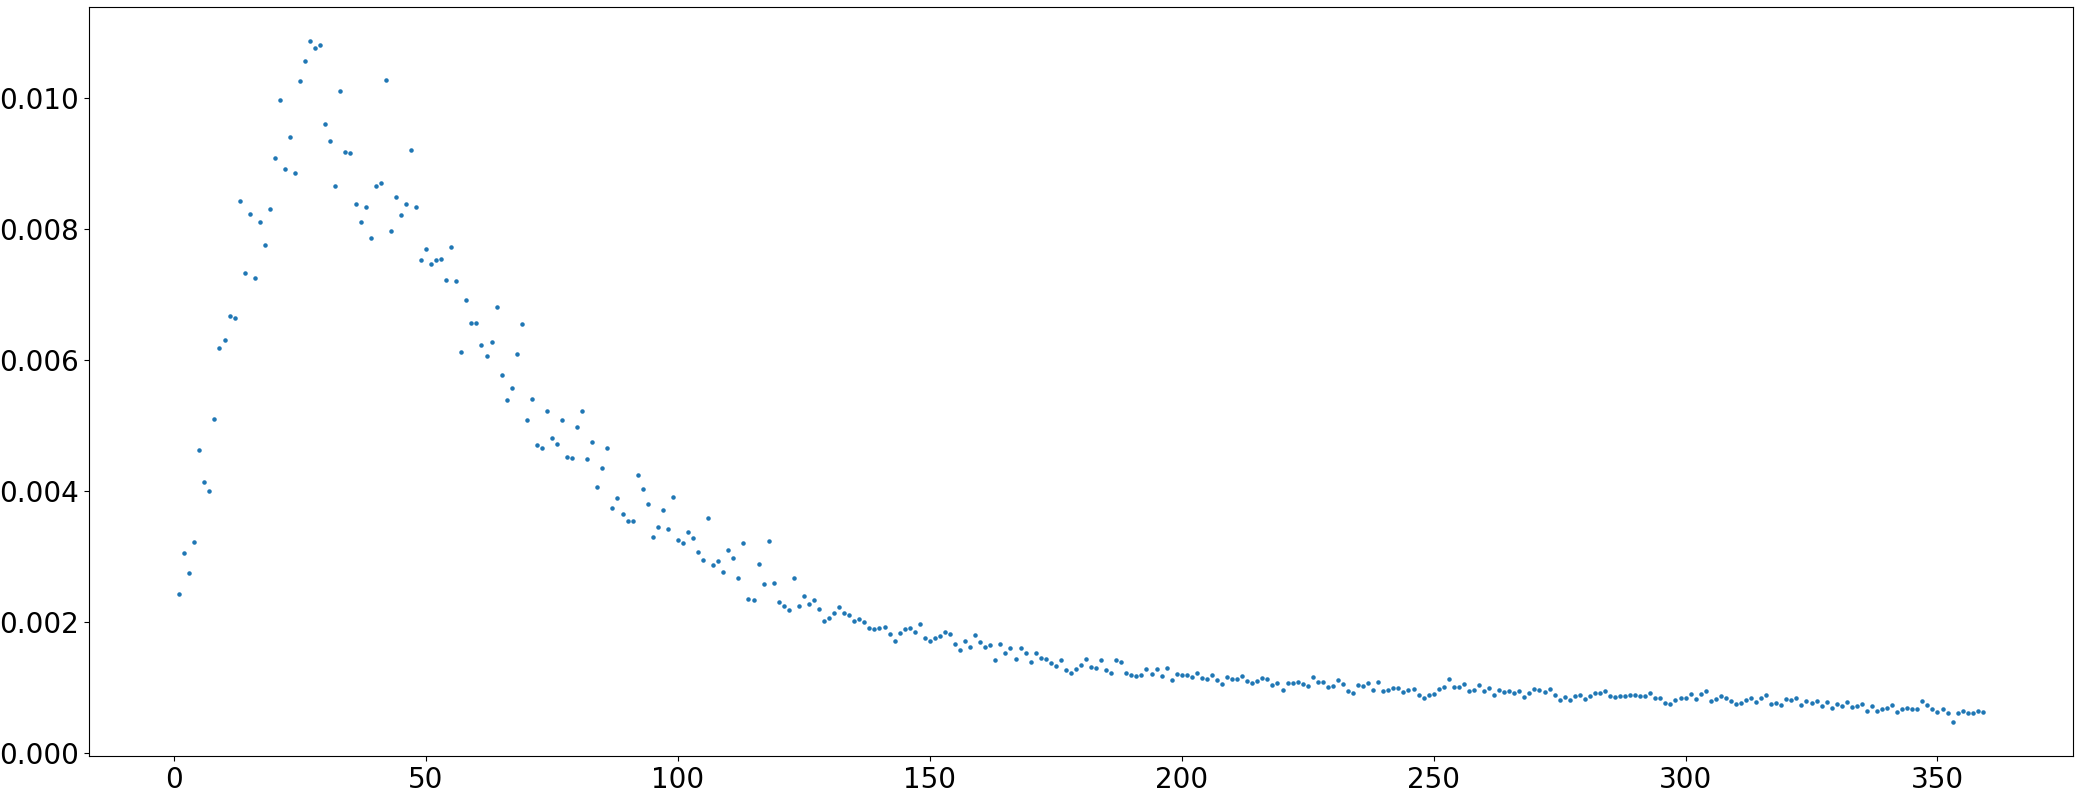
\includegraphics[width=15.5cm]{figures/scatter.png}
    \caption{Original Data Scatter}
    \label{scatter}
\end{figure}

\noindent
Considering the real-world situation and the original data shown in Figure~\ref{scatter}, we adopt the logarithmic normal distribution as the basis of our model. Figure~\ref{log-norm} shows the initial solution using only the Logarithmic Normal Model. It is evident that with Logarithmic Normal Model, there are many errors when talking about report results $200$ days after January 7, 2022. This model cannot successfully estimate the Wordle report results, especially the future results, which is asked in task one.

\begin{figure}[h]
    \centering
    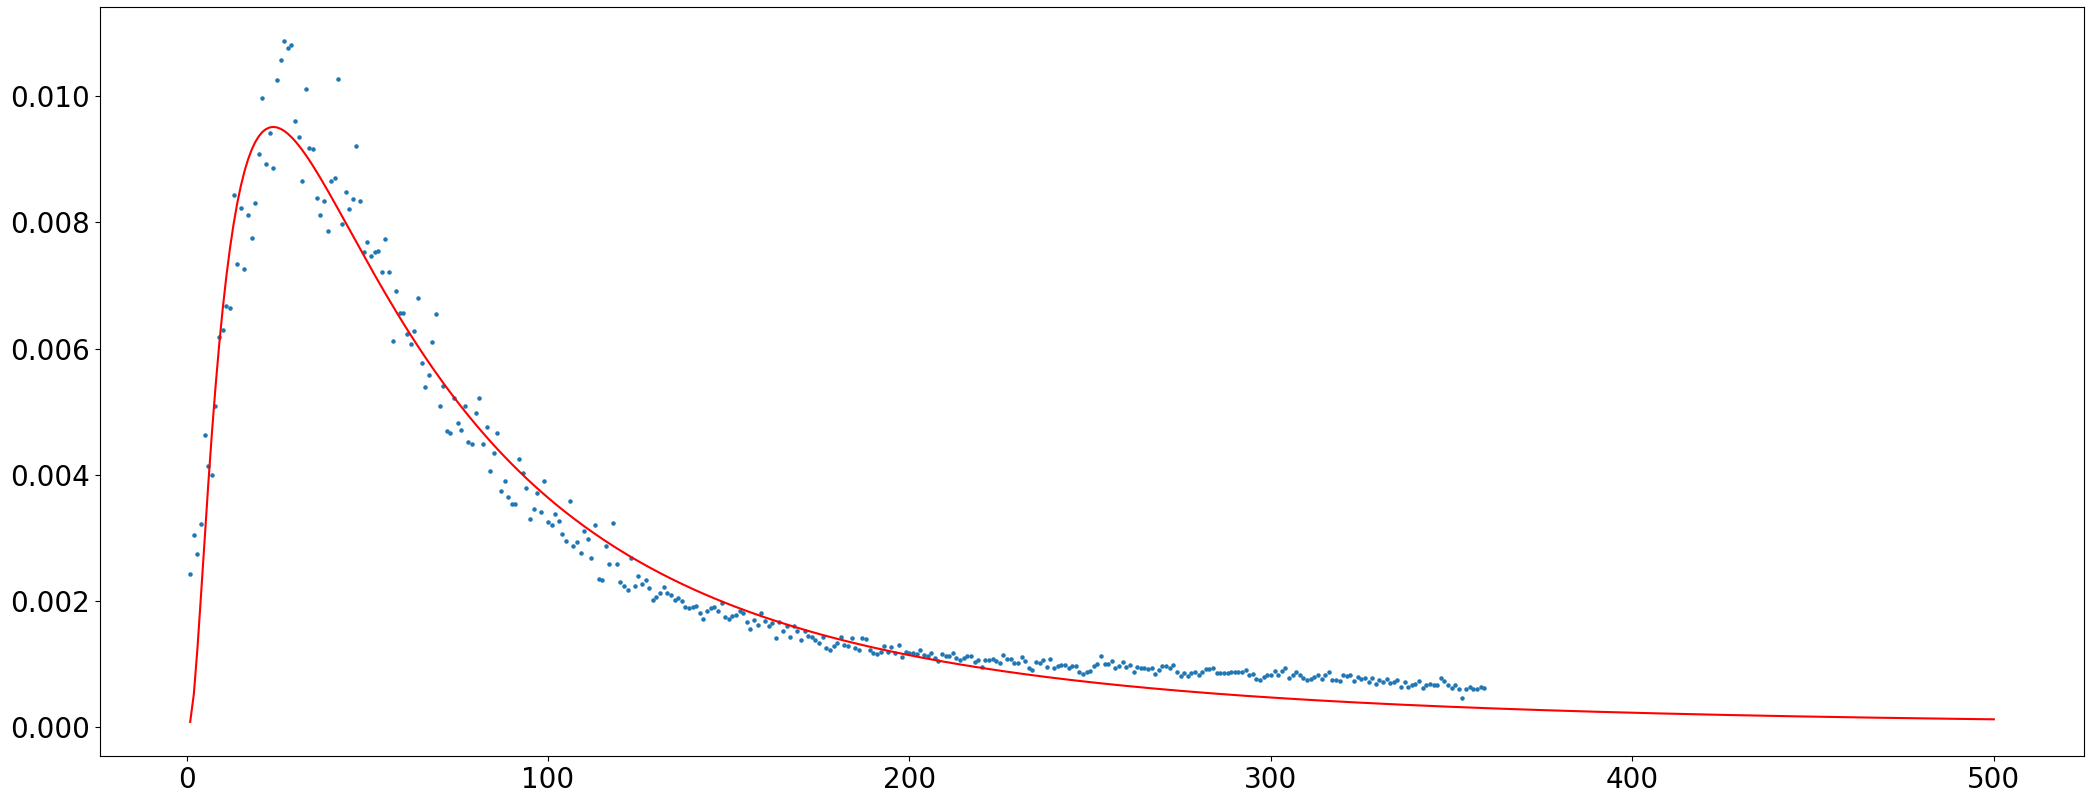
\includegraphics[width=15.5cm]{figures/log-norm.png}
    \caption{Fitting Result with Logarithmic Normal Model}
    \label{log-norm}
\end{figure}

\noindent
In order to eliminate the prediction error, we adjust our model. Based on the knowledge that software has stable users, we add an incremental model consisting of a Logistic Growth Model and a Linear Model. We apply a Logistic Growth Model with initial population $P(0)=100$, with temporary maximum stable user volume $M=10000$, and a growth rate $R=75$. Meanwhile, the Linear Model constantly decreases the stable user volume after $100$ days beyond the start period of the dataset. Figure~\ref{model1Add} displays the relevant result of our improved model, and the green line denotes the incremental component of the model. Table~\ref{table2} and Table~\ref{table3} show the parameters and Root Mean Squared Error (RMSE) of the Logarithmic Normal Model and our Mathematical Time Series Wordle Prediction Model. From the RMSE, we got relatively better results for predicting the report results.

\begin{figure}[h]
    \centering
    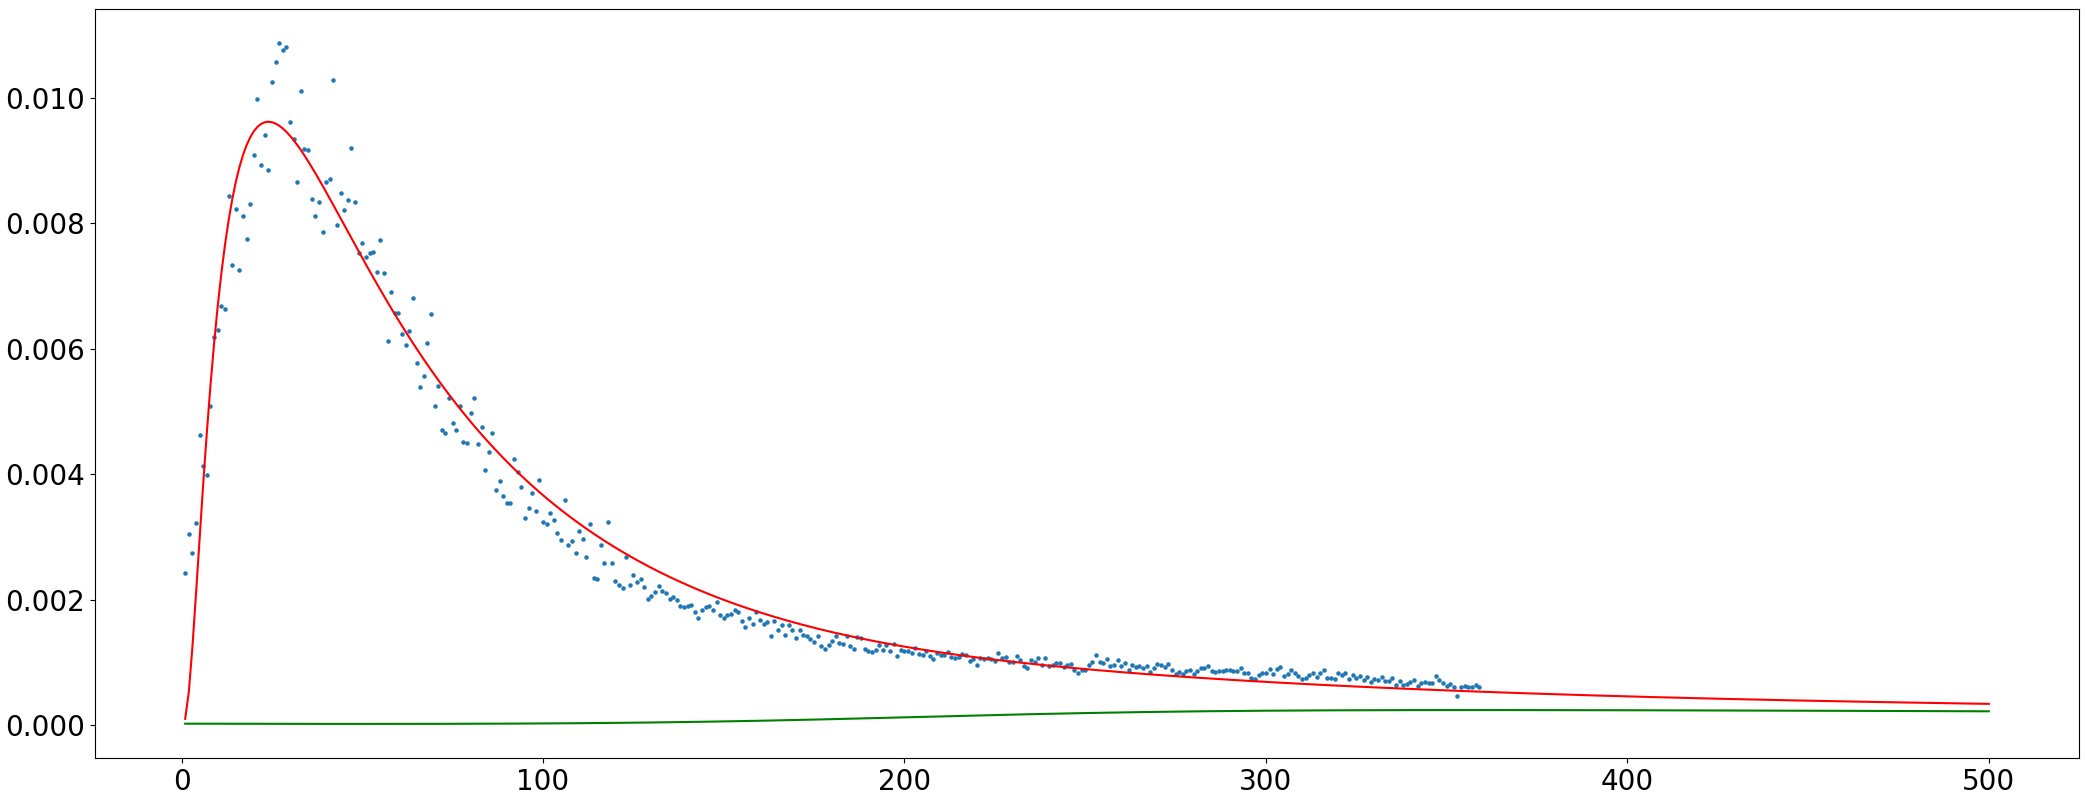
\includegraphics[width=15.5cm]{figures/model1Add.png}
    \caption{Fitting Result with Our Model}
    \label{model1Add}
\end{figure}

\begin{table}[h]
    \centering
    \begin{tabular}{|c|c|}
    \hline
    \textbf{Parameter} & \textbf{Value}     \\ \hline
    $\mu_0$            & 4.236833315740967  \\ \hline
    $\sigma_0$         & 1.0293129975722861 \\ \hline
    RMSE$_0$          & 15369.368407498454 \\ \hline
    \end{tabular}
    \caption{Parameter and RMSE of Logarithmic Normal Model}
    \label{table2}
\end{table}

\begin{table}[h]
    \centering
    \begin{tabular}{|c|c|}
    \hline
    \textbf{Parameter} & \textbf{Value}     \\ \hline
    $\mu_1$            & 4.227476555132943  \\ \hline
    $\sigma_1$         & 1.024076057989859  \\ \hline
    $P(0)$             & 100                \\ \hline
    $M$                & 10000              \\ \hline
    $R$                & 75                 \\ \hline
    $k$                & 0.0000002          \\ \hline
    $x_0$              & 100                \\ \hline
    RMSE$_1$          & 14227.475101826194 \\ \hline
    \end{tabular}
    \caption{Parameter and RMSE of Mathematical Time Series Wordle Prediction Model}
    \label{table3}
\end{table}

\section{Model \uppercase\expandafter{\romannumeral2}}

The concrete embodiment of attributes of the words on the given data is the distribution of the seven groups, representing the number of trials players have done to solve the Wordle problem. The most significant attribute of a word is the order of letters. However, Wordle is not a single permutation and combination problem. Every trial should be a correct English word. Meanwhile, it is hard to quantify this attribute. Thus, the order of letters should not be the primary attribute for us to analyze words in Wordle. Despite the order of letters, the frequency is considered an excellent main attribute of a word to analyze in this game. 

\vspace{0.3cm}
\noindent
We first consider the K-Means Clustering Algorithm (K-Means) based on the Distribution of the Number of Trials (DTNT). Through the model, we classified the words into three different groups. The less guesswork, the easier the word. Then, we construct a Monto Carlo Simulation Model (MCSM) to simulate the process of a person playing Wordle based on the frequency of the word. By repeating the process many times, we could receive a particular distribution of the number of trials of a given the word. To examine the preciseness of the prediction model, we generate the distribution of the number of trials concerning each word that has already appeared in Wordle. From K-value clustering, we obtained the difficulty labeling each word and combined it with our prediction results of the DTNT for each word. We established a Random Forest Classification Model (RFCM). Finally, we calculate Root Mean Square Error (RMSE) to give a fundamental error analysis on our prediction of the word “EERIE”.

\subsection{Limitations Based on the Reported Data}
We analyze the direct correlations between the DTNT and words' frequency. We build a K-means Clustering Model to classify the word according to its DTNT. When we choose k = 3, the clustering center of the three groups shows a significant difference. We rank the groups’ difficulty into easy (E), medium (M), and difficult (D), concerning a numerical rank as 1 (E), 2 (M), and 3 (D). The less guesswork, the easier the word. Then we try to do a regression on the frequency. However, the result shows that the regression model needs to work better. The p-value of each parameter is much greater than 0.05.

\vspace{0.3cm}
\noindent
We summarized the failure and recognized that the Wordle process is a complex combination of independent events. Only the first guess can be viewed as a separate random case. The latter guesses are highly correlated with the former ones. Thus, the Wordle problem needs to be solved numerically and statistically. A logical model of the Wordle process is necessary.

\subsection{Logic of Wordle}

The first selection of the word is random for players, who receive instructional information in a color form. A yellow tile indicates the letter in that tile is in the word but in the wrong location. A green tile indicates that the letter in that tile is in the word and is in the correct location. A gray tile indicates that the letter in that tile is not included in the word. Then players will try another word within the range of words that satisfies the requirement that the instructional information has given. The same goes for steps behind. The process indicates that the times of guesswork depend not only on the words’ frequency but also on the letter formation and order of other words. Thus, to precisely predict a word’s DTNT, we built a logic model to simulate the detailed process for Wordle.

\subsection{Monto Carlo Process for Simulating the Wordle Process}

\subsubsection{Data Preprocessing}

We calculate the probability of selecting a word within a specific range of words by calculating its frequency as a proportion of all word frequencies as following:

$$
P_i=\frac{\text{frequency}_i}{\text{total frequency of word range}} \text{.}
$$

\vspace{0.3cm}
\noindent
Then we construct a probability interval for each word as

$$
\text{Interval}_i=(\sum^{i-1}_{j=1}P_j,\sum^{i}_{j=1}P_j].
$$

\subsubsection{Algorithm}

We first generate seven variables to represent the number of samples with different trials. We construct a judgment algorithm that compares the selected and solution words and outputs the color-formed instructional information. We also construct a selection algorithm that can select words that strictly follow the instructional information from the judgment algorithm.

\vspace{0.3cm}
\noindent
For each simulation, we do the coding following the algorithm below:

\begin{itemize}
    \item {Generate a uniform random variable $x_1$ within the interval $(0,1]$.}

    \item {Select a word whose probability interval contains the value of $x_1$.}

    \item {If the selected word is the solution, add $1$ on the number of samples with one try.}

    \item {If the first selected word is not the solution, while the guess word is not correct:}

    \begin{itemize}
        \item {Select words from the latest range of words using the selection algorithm and update their probability intervals such that the summation of their probabilities equals $1$.}

        \item {Generate a uniform random variable $x_2$ within the interval $(0,1]$.}

        \item {Select a word whose probability interval contains the value of $x_2$.}

        \item {Compare the selected word with the solution with the judgment algorithm.}
    \end{itemize}   

    \item {Record the number of cycles and add $1$ to the variable}
\end{itemize}

\vspace{0.3cm}
\noindent
We allow the number of loops for each word to equal the number of people who participate on that word’s date and calculate the DTNT of each word.

\subsubsection{Adjustment on Data and Algorithm}

In order to simulate a more realistic model, we consider some other behavioral factors based on players' habits when playing Wordle. For instance, players tend to guess a word that is more commonly used and contains more different letters at the first trial. We limit the first guess's word range to the first thousand commonly used words and overweight the words that contain five and four different letters in the first trial. 

\vspace{0.3cm}
\noindent
Also, the word’s frequency cannot directly represent the probability. While the difference in frequency between a commonly-used word and a hardly-used word is too significant. For example, the frequency of the word ABOUT is 1226734006, and the word GAWKY is 31136. It is unrealistic to say that the probability of ABOUT is 39,399 times that of GAWKY. Thus, we try to limit the difference between probabilities to 50 times using the equation below: 

$$
\text{adjustedFrequency}_i=[\log(\text{frequency}_i)]^5
$$

\subsection{Model Assessment}

\subsubsection{Random Forest Classification}
From the previous K-Means clustering, we have a classification of the words based on real-world data. We want to examine if the predicted data can follow the same classification when trained by itself. Thus, we use a Random Forest Classification Model (RFCM) to test the prediction data’s accuracy in classification. RFCM can be directly accessed through the SPSSPRO\cite{spsspro}, an online data analysis platform. We input the class generated by K-means as the nominal level variable and the predicted DTNT, which contains seven variables as a quantitative variable. The training results are shown in Figure~\ref{heatMap} and Table~\ref{table6}.

\begin{figure}[h]
    \centering
    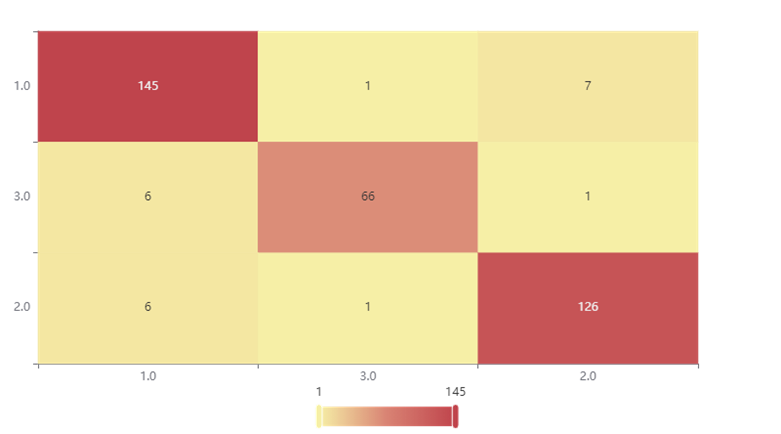
\includegraphics[width=13cm]{figures/heatMap.png}
    \caption{Confusion Matrix Heat Map}
    \label{heatMap}
\end{figure}


\begin{table}[]
    \centering
    \begin{tabular}{|c|c|}
    \hline
    \textbf{Accuracy Rate} & \textbf{Recall Rate} \\ \hline
    93.9\%                 & 93.9\%               \\ \hline
    \end{tabular}
    \caption{Evaluation Result of Model \uppercase\expandafter{\romannumeral2}}
    \label{table6}
\end{table}

\vspace{0.3cm}
\noindent
The RFCM results show that the prediction data’s classification is harmonious with the reported data, which means our simulation model performs well.

\subsubsection{Error Estimation}

In order to give a more flexible prediction of future data on a specific word, we decided to construct data intervals for the predicted DTNT. In case we consider the word into three difficulty classes, by calculating the root of square error between the reported data and the predicted data, denoted by $\sigma_{ij}$, we give different intervals for words that belong to different classes.

$$
\sigma_{ij}=\sqrt{\frac{\sum_{k=1}^n(\text{ReportedPercent}_{ijk}-\text{PredictedPercent}_{ij})^2}{n}},
$$

$$
\text{and Interval}_{ij}=(\text{prediction}-\sigma_{ij},\text{prediction}+\sigma_{ij}).
$$

\vspace{0.3cm}
\noindent
In which $i$ denotes the difficulty classes w.r.t. $i=1(E)$, $2(M)$, $3(D)$, and $j$ denotes the number of steps to guess the solution, which $j=1,2,...,7$.

\section{Model \uppercase\expandafter{\romannumeral3}}

In this section, we proposed a model to classify solution words by difficulty, using the K-Means clustering method and Gaussian Mixture Model (GMM) to make the classification. We compared and chose the better one of these two models to identify the word "EERIE"'s difficulty. 

\vspace{0.3cm}
\noindent
Intuitively speaking, the number of times a player tries can directly reflect how difficult the word is to guess. Since the number of attempts by the player is distributed as an integer between 1 and 6, the number of times greater than or equal to 7 will be counted as 7 times. So we can use clustering algorithms to classify the data from column G to M in the excel file. 

\subsection{Number of Difficulty Levels}
Since too few difficulty levels mean that the model needs to be more accurate to classify the difficulty level, at the same time, too many difficulty levels may make the model over-fitting due to the small amount of data. So we used the Silhouette Coefficient and Rand Index to determine the best number of classification levels using the K-Means algorithm. As Figure~\ref{RI_SC} shows, it is observed that the best choice for it is 3, where both evaluation methods are relatively closer to 1. Therefore, We classified the difficulty into three levels: easy, medium, and difficult in the following part.

\begin{figure}[h]
    \centering
    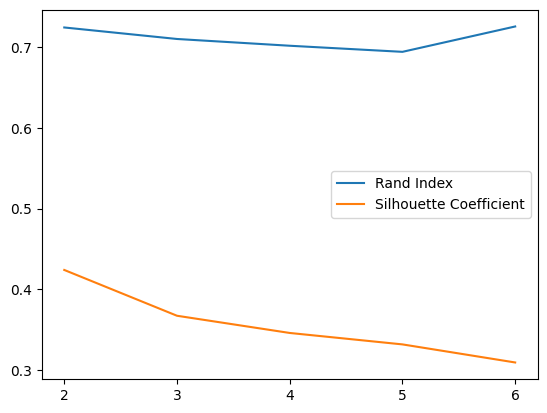
\includegraphics[width=10cm]{figures/RI_SC.png}
    \caption{Silhouette Coefficient and Rand Index w.r.t. Number of Clusters}
    \label{RI_SC}
\end{figure}

\subsection{K-Means and GMM Model}
Using Model \uppercase\expandafter{\romannumeral2}, the attributes of the provided word can be used to predict the distribution of the number of attempts for the original word. Hence we can make classifications on original data and new data generated from the trained model.  
\vspace{0.3cm}
\noindent
The procedure for implementing K-Means Algorithm is shown as follows:

\begin{itemize}
    \item {Choose a specific $K$ denoting the number of clusters, which was optimized to $3$.}

    \item {Randomly put $K$ feature vectors, named centroids, to the feature space.}
    
    \item {Compute the distance from each example $x$ to each centroid $c$ using the Euclidean distance. }

    \item {Label each example with the closest centroid ID.}
    
    \item {Then it becomes the optimization problem:
    $$
    \min_r\sum^n_i\sum^K_kr_{ik}(x_i-c_k)^2 \text{, subject to } r\in\{0,1\}^{n\times K},\sum^K_kr_{ik}=1\text{.}
    $$
    }

    \item {Repeat the following steps:}

    \begin{itemize}
        \item {For each centroid, calculate the average feature vector of the examples labeled. Assign the average feature vectors as the new centroid locations.}

        \item {Recompute the distance from each example to the centroid, modify the assignments, and repeat until they are stable.}
    \end{itemize}

    \item {Calculate the expectation of the distribution of the number of trials on each centroid.}

    \item {Assign the centroid with the largest expectation as “D”, medium as “M”, and the smallest as “E”}
\end{itemize}

\vspace{0.3cm}
\noindent
Compared with K-Means Model, the GMM Model gives a soft margin clustering on the samples. Figure~\ref{clustering} displays each data's clustering result, using k-Means and GMM algorithms. From the figure, it is observed that both algorithms fit the original data well. However, the two difficulty levels share nearly the same tendency and value when the generated data is fit by the GMM method. Therefore, the K-Means algorithm better includes the whole structure. Hence K-means is used for predicting the difficulty levels.

\begin{figure}[h]
    \centering
    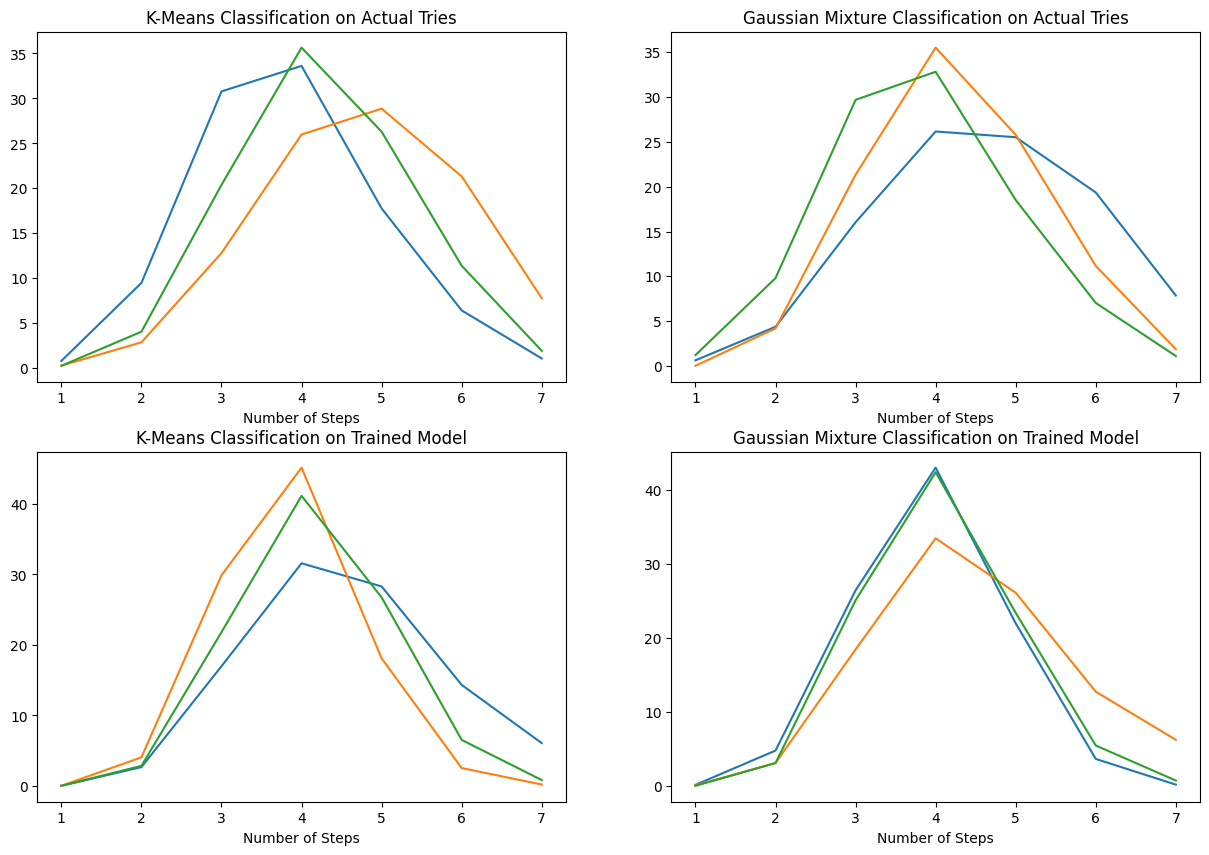
\includegraphics[h]{figures/clustering.png}
    \caption{K-Means and GMM Comparison}
    \label{clustering}
\end{figure}

\subsection{Model Accuracy}
Using Assumption 5,we can measure the difficulty by the average of the trials to guess the solution. The more difficult the word, the more trials are needed. The classification result is shown in Figure\ref{kmeans}.

\begin{figure}[h]
    \centering
    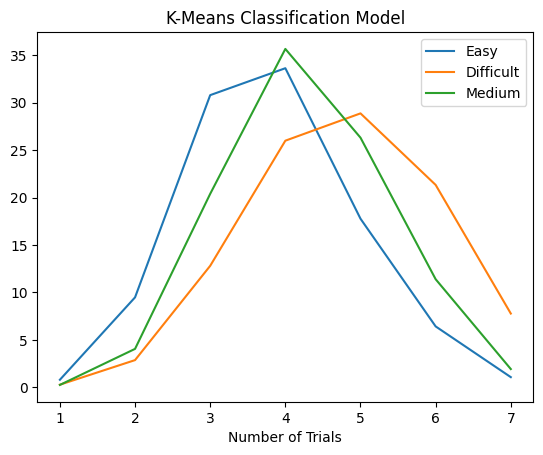
\includegraphics[width=8cm]{figures/kmeans.png}
    \caption{Difficulty of Three Centroids in the K-Means Model}
    \label{kmeans}
\end{figure}

\vspace{0.3cm}
\noindent
Table~\ref{table5} shows the correspondence among colors of curves, average steps, and difficulty levels.

\begin{table}[h]
    \centering
    \begin{tabular}{|c|c|c|}
    \hline
    \textbf{Difficulty} & \textbf{Average Steps} &\textbf{Color}        \\ \hline
    Easy                & 3.8168856375037326     & blue                  \\ \hline
    Medium              & 4.256003684452924      & green                 \\ \hline
    Difficult           & 4.754900616860864      & yellow                \\ \hline
    \end{tabular} 
    \caption{Colors and Average Steps of Each Difficulty}
    \label{table5}
\end{table}

\vspace{0.3cm}
\noindent
Table~\ref{table7} shows the Silhouette Coefficient and Rand Index. The Silhouette Coefficient is calculated using the mean intra-cluster distance $(a)$ and the mean nearest-cluster distance $(b)$ for each sample. The Silhouette Coefficient for a sample is
$(b - a)/\max(a, b)$

\vspace{0.3cm}
\noindent
Since Silhouette Coefficient ranges from -1 to 1, where 1 is the beautiful clustering, our model does not classify it well. However, it is acceptable because there are only six attempts. It is difficult for players to guess the correct answer in the first two trials, and four trials is a mode number. Besides, most players can guess it within six times.  Therefore, the sample data of the three difficulty levels generally have the same trend, and the sample size is not large enough, which results in a relatively small Silhouette Coefficient.

\begin{table}
    \centering
    \begin{tabular}{|c|c|}
    \hline
    \textbf{Parameter} & \textbf{Value}     \\ \hline
    Silhouette Coefficient           & 0.3673287439085649  \\ \hline
    Rand Index                       & 0.710057422075598\\ \hline
    % RMSE$_0$                         & 15369.368407498454 \\ \hline
    \end{tabular}
    \caption{Model Accuracy measured by Silhouette Coefficient and Rand Index}
    \label{table7}
\end{table}

\clearpage

\section{Conclusion}

\subsection{Solution}

\subsubsection{Task 1}
According to our Mathematical Time Series Wordle Prediction Model, we can predict the number of the reported result on March 1, 2023, which is 14377. Several word attributes affect the percentage of scores played in Hard Mode. For instance, with the decrease in word frequency, the rate of finishing the game with fewer tries will decrease. Also, particular prefixes and suffixes like ”ab-” or ”-st” will reduce the difficulty of the game, which leads to an increase in the percentage of finishing the game with fewer tries. Some high-frequency letters like ”a”, ”e” in words also influence the distribution of report results. However, the pattern of those letters has different effects on the results. For instance, ”mummy” is a problematic word in the game, although it has a relatively high word frequency.

\subsubsection{Task 2}
Our model's prediction shows that the proportion of players who can solve the Wordle problem in 1 trial is always less than $0.1\%$. However, the reported result shows that the proportion of many words' 1 trial success can reach $1\%$ or even larger. We consider this bias caused by our assumption 2 that all players are honest, which may not be valid. Thus, our model may need to be more accurate in predicting on both 1 try and 7 or more trials. Moreover, as time passes, the left players are considered more experienced, which means their skills on Wordle may lead to smaller intermediate steps to guess the solution. However, it is a feature that is hard to quantify. We only consider a two-period comparison. The players might be cleverer in the future.
The prediction results of "EERIE" is shown in Table~\ref{table8}:

\begin{table}[h]
    \centering
    \begin{tabular}{|c|c|c|c|c|c|c|c|}
    \hline
    \textbf{}       & \textbf{1 try} & \textbf{2 tries} & \textbf{3 tries} & \textbf{4 tries} & \textbf{5 tries} & \textbf{6 tries} & \textbf{7 or more tries} \\ \hline
    \textbf{Result} & 0              & 1.9\%            & 17.1\%           & 40.5\%           & 31.5\%           & 7.5\%            & 1.2\%                    \\ \hline
    \textbf{STD}    & 0.7            & 0.51             & 1.25             & 2.75             & 2.94             & 1.25             & 0.62                     \\ \hline
    \end{tabular}
    \caption{Prediction of EERIE Report Distribution}
    \label{table8}
\end{table}

\subsubsection{Task 3}
The best cluster number is 3, optimized using Rand Index and Silhouette Coefficient. Then we classify the difficulty into three levels: D, MD, and E. After comparing the accuracy of the K-Means and GMM models. We conclude that the K-Means model better fits the sample data. Using the cluster centers from the K-Means model and the above prediction distribution of "ERRIE," we classify the difficulty of "ERRIE" as Medium Difficult. Our model has a moderate rand index, which falls from 0.65 to 0.8, which can predict the difficulty well. However, our model does not have a high Silhouette Coefficient, which means that the instances in the cluster are compact, and part of the instances overlap to some extent. 

\subsubsection{Task 4}

\begin{itemize}
    \item {Several words have an abnormally high one-try successful rate, which our model cannot fit well.}

    \item {There are words with high failure rates. For instance, in position M108, 48\% of players can only solve the puzzle in up to six tries.}

    \item {The percentage of Hard Mode players continues to rise and holds steady at $10\%$ in around the last 100 days of the report. This trend shows an increase in the proportion of experienced players.}
\end{itemize}

\subsection{Overall Evaluation}

\subsubsection{Strengths}

For Model \uppercase\expandafter{\romannumeral1}, we use the natural world approach to fit the dataset, which considers there is a "stable user group" to support the total user volume. Also, we apply a constantly decreased linear model to represent the user churn as the software develops. For Model \uppercase\expandafter{\romannumeral2}, we develop a logical model to simulate the Wordle process for a specific word, which allows us to give a reasonable distribution for each word within the word range. We make some adjustments to the data and algorithm in consideration of realistic situations. We also view the reported distribution as the manifestation of difficulty and use it to do K-means Clustering, giving the words a particular class. After predicting the DTNT of every word that has already appeared in Wordle, we use the predicting data as a quantitative variable and the class given by K-means as the nominal level variable to operate Random Forest Classification to verify the accuracy of our model's prediction. The combination of two machine learning algorithms enhances the model's robustness. For Model \uppercase\expandafter{\romannumeral3}, we optimize the number of clusters to 3 to ensure higher accuracy and convenience. Also, our clustering results generate relatively fitting curves w.r.t the reporting data.

\subsubsection{Weaknesses}

However, for Model \uppercase\expandafter{\romannumeral1}, since we are using the mathematical method to estimate the results, we cannot fully cover the trends of the reporting results. For instance, the weekly fluctuation due to the Working Days and Rest Days, and the festivals effects are ignored in our model. For Model \uppercase\expandafter{\romannumeral2}, our simulation model's bias mainly comes from our assumptions 1 and 2. These two assumptions has eliminated a lot of uncertain variables for the model. Those behavioral variables are too complex to be quantified. For Model \uppercase\expandafter{\romannumeral3}, our clustering curves follow the same trend, which decreases the classification accuracy and inevitably influences our model. Meanwhile, after predicting the results, the clustering model cannot distinguish efficiently, increasing our classification's difficulty.

\subsubsection{Future Work}

\begin{itemize}
    \item {Due to the time limit, many potential attributes will influence the distribution of the dataset. Also, the limited sample size restricts our models' performance—more data is needed in the future. }

    \item {Since the gaming results depend primarily on the first several guesses, we can study deeper on this determined aspect to better predict the result distribution.}

    \item {Despite only analyzing the influence of word frequency, we can take information entropy into account to simulate the thinking process of the human brain.}
\end{itemize}

\clearpage

\section{A Letter to the Puzzle Editor}

Dear Editor,

\vspace{0.1cm}
\noindent
Following your instructions, we analyzed the data in the file you provided and the dictionary data from Kaggle. We constructed different mathematical models to answer the first three question sets. The first is a Mathematical Time Series Wordle Prediction Model, a combination of the Logarithmic Normal and Logistic Growth Model. The second one is a Monte Carlo Simulation Model for the Wordle process. The third one contains K-means Model and GMM Model. The detailed report is as follows.

\vspace{0.1cm}
\noindent
\textbf{For the first question set}, as we drew the scatter graph of the number of reported players along the time series, we observed that the data’s shape is close to the probability density function (PDF) of the logarithmic normal distribution. Then we write a function fitting code to establish a Logarithmic Normal Model to fit the initial data. By changing the parameter of the function curve, we received a result in Figure~\ref{letterlog-norm}. This result is ideal in the first 200 days but obtained a significant decrease compared to the reported data. Thus, we introduced a new concept, the “stable users”. We assume that the group of stable users follows a logistic growth and add a curve generated by the Logistic Growth Model. After fitting the new model, we received a more precise visual and numerical prediction result. Details are shown in Figure~\ref{lettermodel1Add} below. The final result of our prediction is that we will receive data from 14377 players. 

\begin{figure}[h]
    \centering
    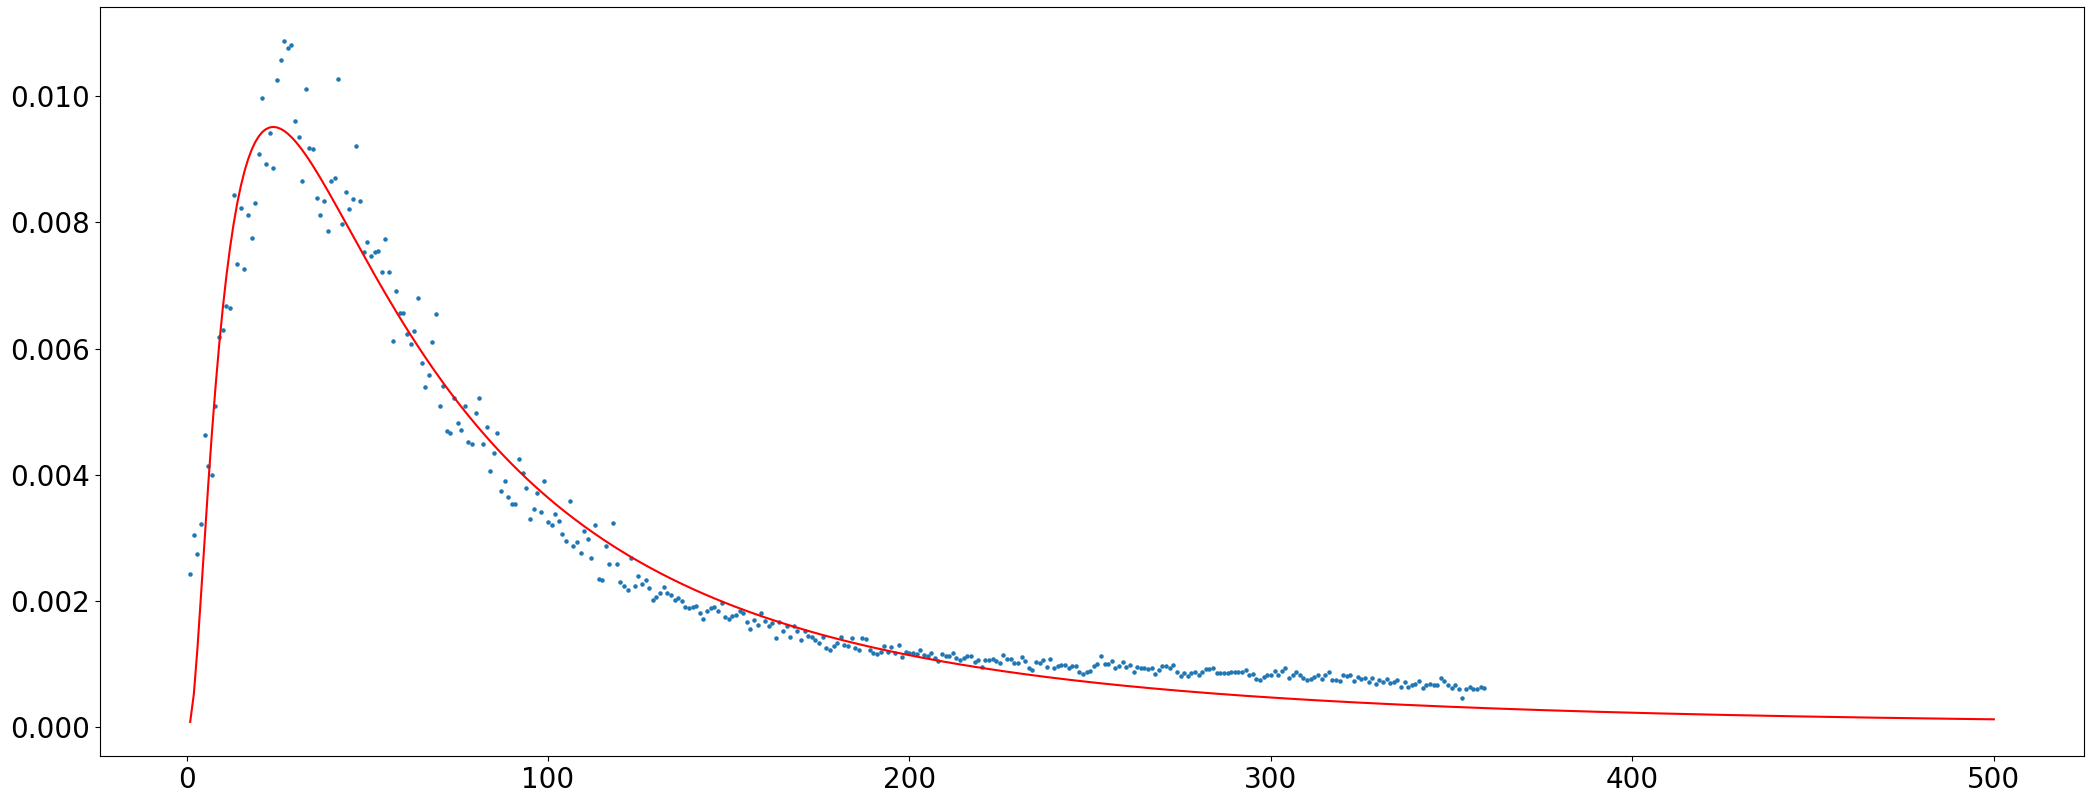
\includegraphics[width=10cm]{figures/log-norm.png}
    \caption{Fitting Result with Our Model}
    \label{letterlog-norm}
\end{figure}

\begin{figure}[h]
    \centering
    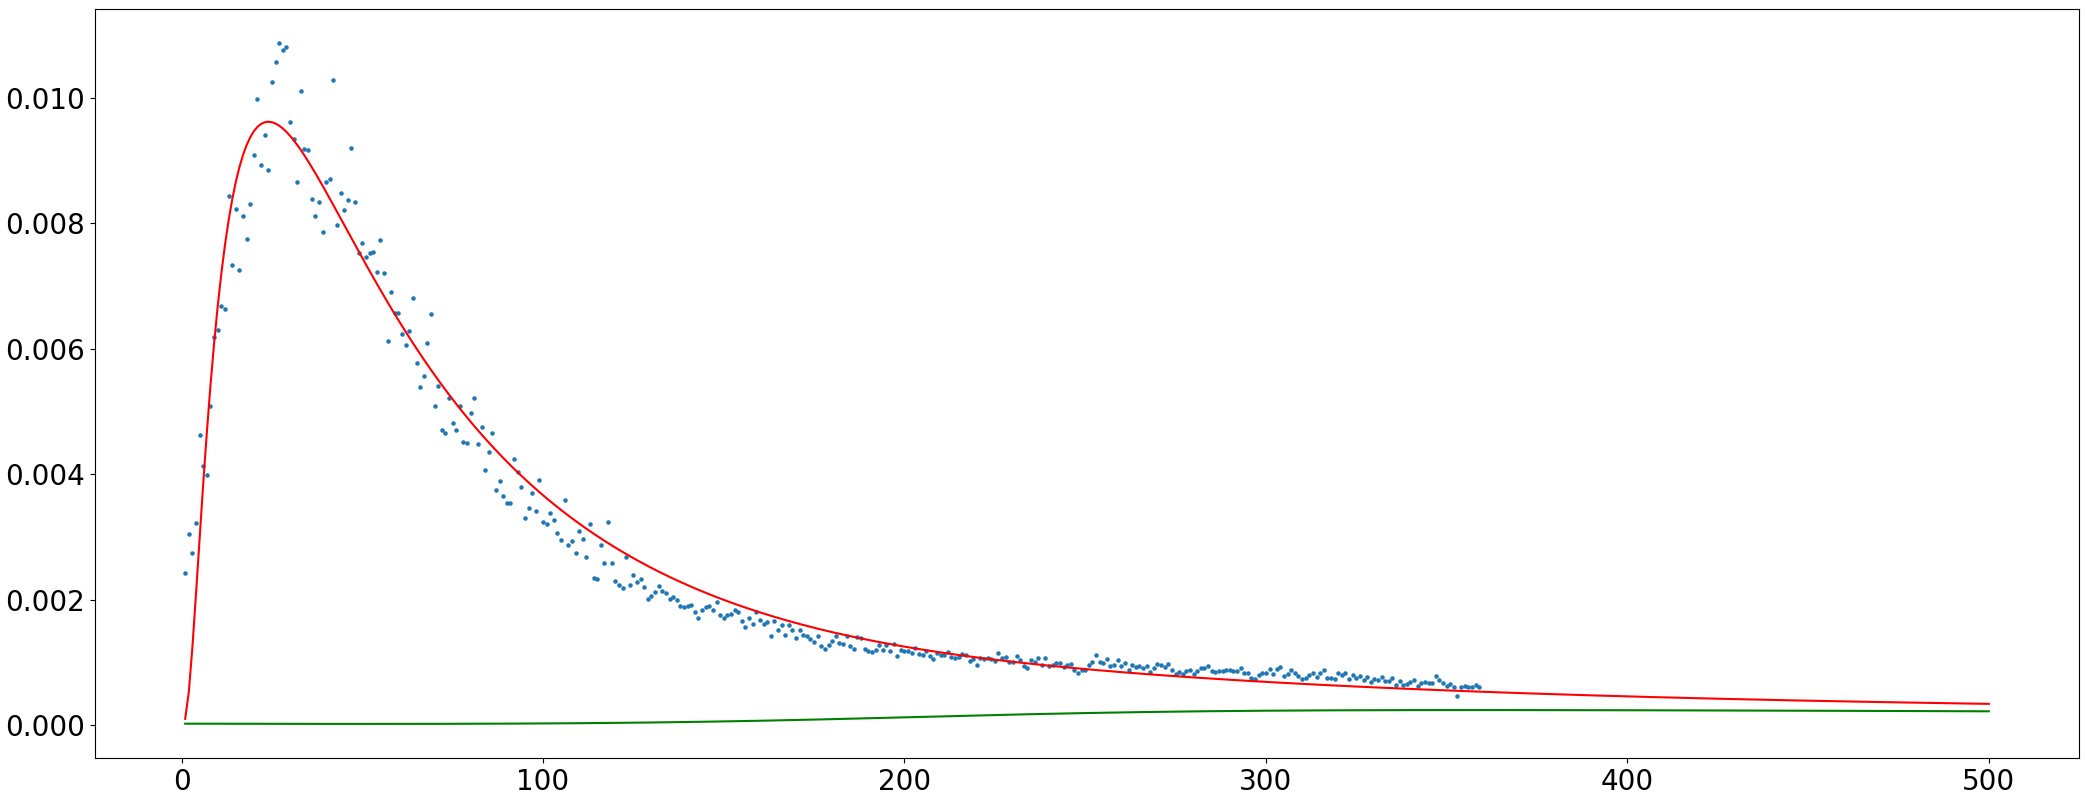
\includegraphics[width=10cm]{figures/model1Add.png}
    \caption{Fitting Result with Our Model}
    \label{lettermodel1Add}
\end{figure}

\vspace{0.1cm}
\noindent
Several attributes of the word affect the percentage of scores reported that were played in Hard Mode. For instance, with the decrease in word frequency, the percentage of finishing the game with fewer tries will decrease. Also, for a specific prefix and suffix like "ab-" or "-st", it will reduce the difficulty of the game, which leads to an increase in the percentage of finishing the game with fewer tries. Moreover, high-frequency letters like "a", "e" in words also influence the distribution of report results.  However, the pattern of those letters has different effects on the results. For instance, "mummy" is a problematic word in the game, although it has a relatively high word frequency.

\vspace{0.1cm}
\noindent
\textbf{For the second question set}, we needed help building a model that only analyzes the data numerically and statistically.Then we wrote down the detailed logic of the Wordle process and established a Monte Carlo Simulation Model (MCSM) to simulate the game process precisely. Once we input a particular word and cycle index, it returns a percentage distribution of the number of trials. For the word EERIE that you required, we used the predicted result from the first model that there will be 14377 players’ data on March 1st, 2023 as the cycle index. By running the MCSM, we received a result as Table~\ref{letterTable}.

\begin{table}[h]
    \centering
    \begin{tabular}{|c|c|c|c|c|c|c|c|}
    \hline
    \textbf{}       & \textbf{1 try} & \textbf{2 tries} & \textbf{3 tries} & \textbf{4 tries} & \textbf{5 tries} & \textbf{6 tries} & \textbf{7 or more tries} \\ \hline
    \textbf{Result} & 0              & 1.9\%            & 17.1\%           & 40.5\%           & 31.5\%           & 7.5\%            & 1.2\%                    \\ \hline
    \textbf{STD}    & 0.7            & 0.51             & 1.25             & 2.75             & 2.94             & 1.25             & 0.62                     \\ \hline
    \end{tabular}
    \caption{Prediction of EERIE Report Distribution}
    \label{letterTable}
\end{table}

\vspace{0.1cm}
\noindent
To test the preciseness of our model, we use K-means Clustering to classify the reported data into three groups. Then we run a Random Forest Classification Model based on the prediction data, which contains all the words appearing in the given reported data. The results of the two classification models show significant homogeneity. Thus, we are confident in our prediction results. The uncertainties of our model may be the bias caused by our assumptions 1 and 2, which may not be accurate as players are not so efficient in playing the game as our MCSM do and might need to be more honest when they report their grades.

\vspace{0.1cm}
\noindent
\textbf{For the third question set}, we found the optimal number of clusters equaled three, where both overfitting and underfitting were well avoided. Moreover, when clustering the distribution of the number of trials, using the K-Means model rather than Gaussian Mixture Model is better. Since there were overlaps in the number of trial distributions, the Silhouette Coefficient wouldn’t be large enough, while the Rand Index remained high.

\vspace{0.1cm}
\noindent
\textbf{For the fourth question set}, we proposed three interesting data set features. For instance, several words have an abnormally high one-try successful rate, which our model cannot fit well. And there are words with high failure rates. For instance, in position M108, 48\% of players can only solve the puzzle in up to six tries. Also, the percentage of Hard Mode players continues to rise and holds steady at $10\%$ in around the last 100 days of the report. This trend shows an increase in the proportion of experienced players.

\vspace{0.1cm}
\noindent
The above is the entire content of our models. Should you need more information, we'll gladly discuss our investment strategy models in detail at the next meeting.

\vspace{0.1cm}
\noindent
\rightline{\textbf{Sincerely,}}
\rightline{\textbf{Team 2322161}}

\clearpage
\bibliographystyle{unsrt}  
\bibliography{reference}
\end{document}